\documentclass[a4paper, 12pt]{article}

\usepackage{exercise-sheet}
\usepackage{global-macros}
\usepackage{biblatex}
\usepackage{csquotes}
\usepackage{hyperref}
\usepackage{graphicx}
\graphicspath{{../fig}}
\usepackage{float}

% \usepackage[nomarkers]{endfloat}

\hfuzz=16pt

\addbibresource{../bib/references.bib}

\title{Aprendizado de Máquinas -- Avaliação 1} 
\author{Professor: Rodrigo Targino \\
        Aluno: Caio Lins}
\date{\today}

\begin{document}

\maketitle

\section{Apresentação do Dataset}

Como banco de dados para ser utilizado no projeto final da disciplina, escolhemos o \emph{``Census Income Data Set''}\cite{uci}.
O dataset foi extraído da base de dados do censo populacional americano de 1994.
Cada instância representa um indivíduo, que possui algumas caracteríscas sociais e econômicas disponíveis, correspondentes às colunas da tabela.
Os dados foram extraídos já com um problema de classificação binária em mente: a coluna relativa à renda anual do indivíduo só informa se ele ganha mais ou menos que \$50 000 por ano.
Nosso objetivo será ajustar modelos de classificação a esses dados, de modo a classificar um dado indivíduo com relação ao seu salário, baseando-nos nas outras variáveis disponíveis.
Nessa primeira parte, faremos uma análise exploratória dos dados, discutindo suas principais características.

\subsection{Descrição das variáveis}

Para ler e manipular os dados, utilizamos a versão 1.2.4. da biblioteca \emph{Pandas} \cite{pandas}, da linguagem de programção \emph{Python} \cite{python}, versão 3.8.10.
No repositório da UCI, os dados se encontram previamente dividos em um conjunto para treino e outro para teste, na proporção 2:1.
Nós juntamos as duas tabelas para obter um data frame com todas as instâncias disponíveis.
No total, são 48 840 entradas com 15 atributos distintos, listados a seguir:

\begin{itemize}
    \item \verb|Age|.
        Variável numérica que assume valores inteiros.
        Corresponde à idade do indivíduo.

    \item \verb|workclass|.
        Variável categórica que assume os seguintes valores:
        \verb|Private|, \verb|Self-emp-not-inc|, \verb|Self-em-inc|, \verb|Local-gov|, \verb|State-gov|, \verb|Federal-gov|, \verb|Without-pay|, \verb|Never-worked|.
        Corresponde a uma classificação do emprego do indivíduo, com relação ao tipo de vínculo empregatício.

    \item \verb|fnlwgt|.
        Variável numérica que assume valores inteiros.
        É um peso calculado pelo \href{https://www.census.gov/programs-surveys/cps/technical-documentation/methodology/weighting.html}{\emph{United States Census Bureau}} que indica quantas pessoas aquele indivíduo representa na população .
        Ele é necessário para realizar inferências sobre a população toda do país, devido às estratégias de amostragem utilizadas para decidir quem será entrevistado no censo.

    \item \verb|education|.
        Variável categórica que assume os seguintes valores:
        \verb|Preschool|, \verb|1st-4th|, \verb|5th-6th|, \verb|7th-8th|, \verb|9th|, \verb|10th|, \verb|11th|, \verb|12th|, \verb|HS-grad|, \verb|Some-college|, \verb|Assoc-voc|, \verb|Assoc-acdm|, \verb|Bachelors|, \verb|Masters|, \verb|Prof-school|, \verb|Doctorate|.
        Corresponde ao grau máximo de educação obtido pelo indivíduo.

    \item \verb|education_num|.
        Variável numérica que assume valores inteiros entre 1 e 16.
        Corresponde a uma codificação numérica da educação do indivíduo, na ordem apresentada na descrição da variável \verb|education|.
        Não está claro o que alguns valores que \verb|education| assume significam, como, por exemplo, \verb|Assoc-voc| ou \verb|Assoc-acdm|.
        Com isso, não temos total certeza que a variável \verb|education| é ordenável.
        Entretanto, vamos supor que ela é, justamente por causa dessa ordenação que foi disponibilizada junto com o dataset.

    \item \verb|marital_status|.
        Variável categórica que assume os seguintes valores:
        \verb|Married-civ-spouse|, \verb|Divorced|, \verb|Never-married|, \verb|Separated|, \verb|Widowed|, \verb|Married-spouse-absent|, \verb|Married-AF-spouse|.
        Corresponde à situação conjugal do indivíduo.

    \item \verb|occupation|.
        Variável categórica que assume os seguintes valores:
        \verb|Tech-support|, \verb|Craft-repair|, \verb|Other-service|, \verb|Sales|, \verb|Exec-managerial|, \verb|Prof-specialty|, \verb|Handlers-cleaners|, \verb|Machine-op-inspct|, \verb|Adm-clerical|, \verb|Farming-fishing|, \verb|Transport-moving|, \verb|Priv-house-serv|, \verb|Protective-serv|, \verb|Armed-Forces|.
       Corresponde a uma classificação do emprego do indivíduo com relação ao tipo de atividade exercida.
       
    \item \verb|relationship|.
        Variável categórica que assume os seguintes valores:
        \verb|Wife|, \verb|Own-child|, \verb|Husband|, \verb|Not-in-family|, \verb|Other-relative|, \verb|Unmarried|.
        Corresponde a uma classificação das relações familiares mais próximas do inidivíduo.

    \item \verb|race|.
        Variável categórica que assume os seguintes valores:
        \verb|White|, \verb|Black|, \verb|Asian-Pac-Islander|, \verb|Amer-Indian-Eskimo|, \verb|Other|.
        Corresponde à raça do indivíduo.

    \item \verb|sex|.
        Variável categórica que assume os seguintes valores:
        \verb|Male|, \verb|Female|.
        Corresponde ao sexo do indivíduo.

    \item \verb|capital_gain|.
        Variável numérica que assume valores inteiros.
        Não há uma descrição precisa do que essa variável significa na página do dataset.
        Entretanto, pelo nome dela pode-se inferir que se trata de algum ganho monetário não diretamente relacionado ao salário anual do indivíduo.

    \item \verb|capital_loss|.
        Variável numérica que assume valores inteiros.
        Não há uma descrição precisa do que essa variável significa na página do dataset.
        Entretanto, pelo nome dela pode-se inferir que se trata de uma perda monetária não diretamente relacionada ao salário anual do indivíduo.

    \item \verb|hours_per_week|.
        Variável numérica que assume valores inteiros.
        Corresponde ao número de horas semanais que o indivíduo passa trabalhando.

    \item \verb|native_country|.
        Variável categórica que corresponde ao país onde o indivíduo nasceu.
        Há muitos valores possíveis para essa variável para citá-los todos.

    \item \verb|target|.
        Variável categórica que corresponde à renda anual do indivíuo.
        Ela assume os valores \verb|<=50K| e \verb|>50K|.

\end{itemize}

Infelizmente, a descrição dos dados fornecida na página da UCI não é muito detalhada, e a base de dados original do censo de 1994 não está mais disponível no website do \emph{United States Census Bureau}.
Com isso, não está muito claro o que alguns valores assumidos por variáveis categóricas significam.
Isso pode dificultar a interpretação das análises futuras.

Algumas estatísticas descritivas para as variáveis numéricas são apresentadas na Tabela \ref{tab: describe}.
\begin{table}
    \begin{center}
        \begin{tabular}{lrrrr}
        {} &           \verb|age| &  \verb|education_num| &  \verb|capital_gain| &  \verb|capital_loss| \\
        \hline
        mean  &     38.643857 &      10.078092 &   1079.067301 &     87.505897 \\
        std   &     13.710652 &       2.570954 &   7452.168393 &    403.012415 \\
        min   &     17.000000 &       1.000000 &      0.000000 &      0.000000 \\
        25\%   &     28.000000 &       9.000000 &      0.000000 &      0.000000 \\
        50\%   &     37.000000 &      10.000000 &      0.000000 &      0.000000 \\
        75\%   &     48.000000 &      12.000000 &      0.000000 &      0.000000 \\
        max   &     90.000000 &      16.000000 &  99999.000000 &   4356.000000 \\
        \hline
        \end{tabular}
    \end{center}

    \hspace{2.4cm}
    \begin{tabular}{lrr}
    {} &  \verb|hours_per_week| &        \verb|target| \\
    \hline
    mean  &       40.422400 &      0.239292 \\
    std   &       12.391697 &      0.426655 \\
    min   &        1.000000 &      0.000000 \\
    25\%   &       40.000000 &      0.000000 \\
    50\%   &       40.000000 &      0.000000 \\
    75\%   &       45.000000 &      0.000000 \\
    max   &       99.000000 &      1.000000 \\
    \hline
    \end{tabular}
    \label{tab: describe}
    \caption{Estatísticas descritivas para as variáveis numéricas do dataset.}
\end{table}
É interessante observar a probabilidade de um indivíduo ganhar mais de \$50 000 por ano, sem nenhuma informação adicional: 23.92 \%.
Também vemos que os indivíduos têm, em média, 38.6 anos de idade e trabalham 40 horas por semana, o que está dentro do que se espera para a população economicamente ativa de um país.

\subsection{Tratamento realizado}

Além de juntar os datasets disponibilizados no repositório da UCI, foi necessário formatar as entradas da tabela que são strings, para retirar um espaço em branco que estava no início de todas elas.
Também mudamos a variável \verb|target| para que assumisse os valores \( 1 \), se o indivíduo ganha mais de \$50 000 por ano, e \( 0 \) se não ganha e transformamos as variáveis categóricas não ordenáveis em indicadoras.

Tomamos a decisão de remover a coluna \verb|fnlwgt|, pois o peso atribuído a cada indivíduo só é útil quando o objetivo é fazer inferências para toda a população americana.
Como estamos mais interessados em aplicar modelos preditivos apenas na amostra incompleta presente no nosso dataset, essa variável não é relevante, pois sabemos que ela não influencia a variável \verb|target|.

É claro, mas vale ressaltar, que quando formos ajustar modelos aos nossos dados, não vamos utilizar, simultaneamente, as informações das colunas \verb|education| e \verb|education_num|, por serem, do ponto de vista informacional, idênticas.


Com relação a dados faltantes, apenas três colunas apresentam essa característica, como podemos ver na Tabela \ref{tab: missing_data}.
\begin{table}
    \centering
    \begin{tabular}{l|c}
        Atributo & Número de entradas faltantes \\
        \hline
        \verb|workclass| & 2799 \\
        \verb|occupation| & 2809 \\
        \verb|native_country| & 857 \\
    \end{tabular}
    \label{tab: missing_data}
    \caption{Número de dados faltantes.}
\end{table}
Como a quantidade de dados faltantes é pequena em relação ao total de instâncias no conjunto de dados, descartar os indivíduos sem informação completa é uma estratégia viável para conseguir aplicar modelos de classificação.
Entretanto, isso pode não ser necessário, e essa decisão não será tomada neste ponto da análise.

\section{Estudo das relações entre as variáveis}

Vamos começar analisando as correlações entre as variáveis numéricas disponíveis, apresentadas na Figura \ref{fig: corr}.

\begin{figure}[htb]
    \begin{center}
        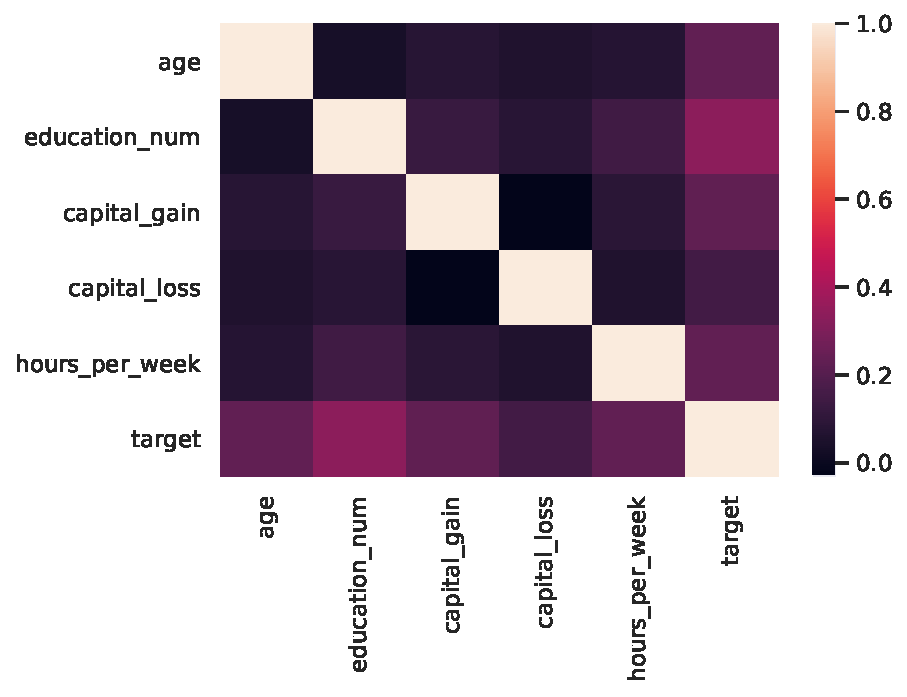
\includegraphics[width=.6\textwidth]{correlation.pdf}
    \end{center}
    \caption{Correlações entre as variáveis numéricas do dataset.}
    \label{fig: corr}
\end{figure}

Vemos que, no geral, as elas não são muito correlacionadas, especialmente as variáveis preditoras entre si.
Os maiores coeficientes obtidos foram para as correlações que envolviam a variável independente, sendo que o maior deles foi \( 0.332624 \), com a variável \verb|education_num|.
Isso indica que, em geral, indivíduos com maior escolaridade têm um salário mais elevado.
É interessante observar que a variável \verb|capital_loss| possui uma correlação \emph{positiva} com \verb|target|, o que é não é intuitivo, considerando seu nome.
Isso nos faz questionar qual o real significado desas variável.

Também fizemos um plot contendo as correlações entre todas as variáveis (incluindo indicadoras) e o \verb|target|, apresentado na Figura \ref{fig: corr target}.
Como são muitas categorias, selecionamos apenas aquelas que apresentaram um valor absoluto de correlação amostral maior que \( 0.2 \).
\begin{figure}[htb]
    \begin{center}
        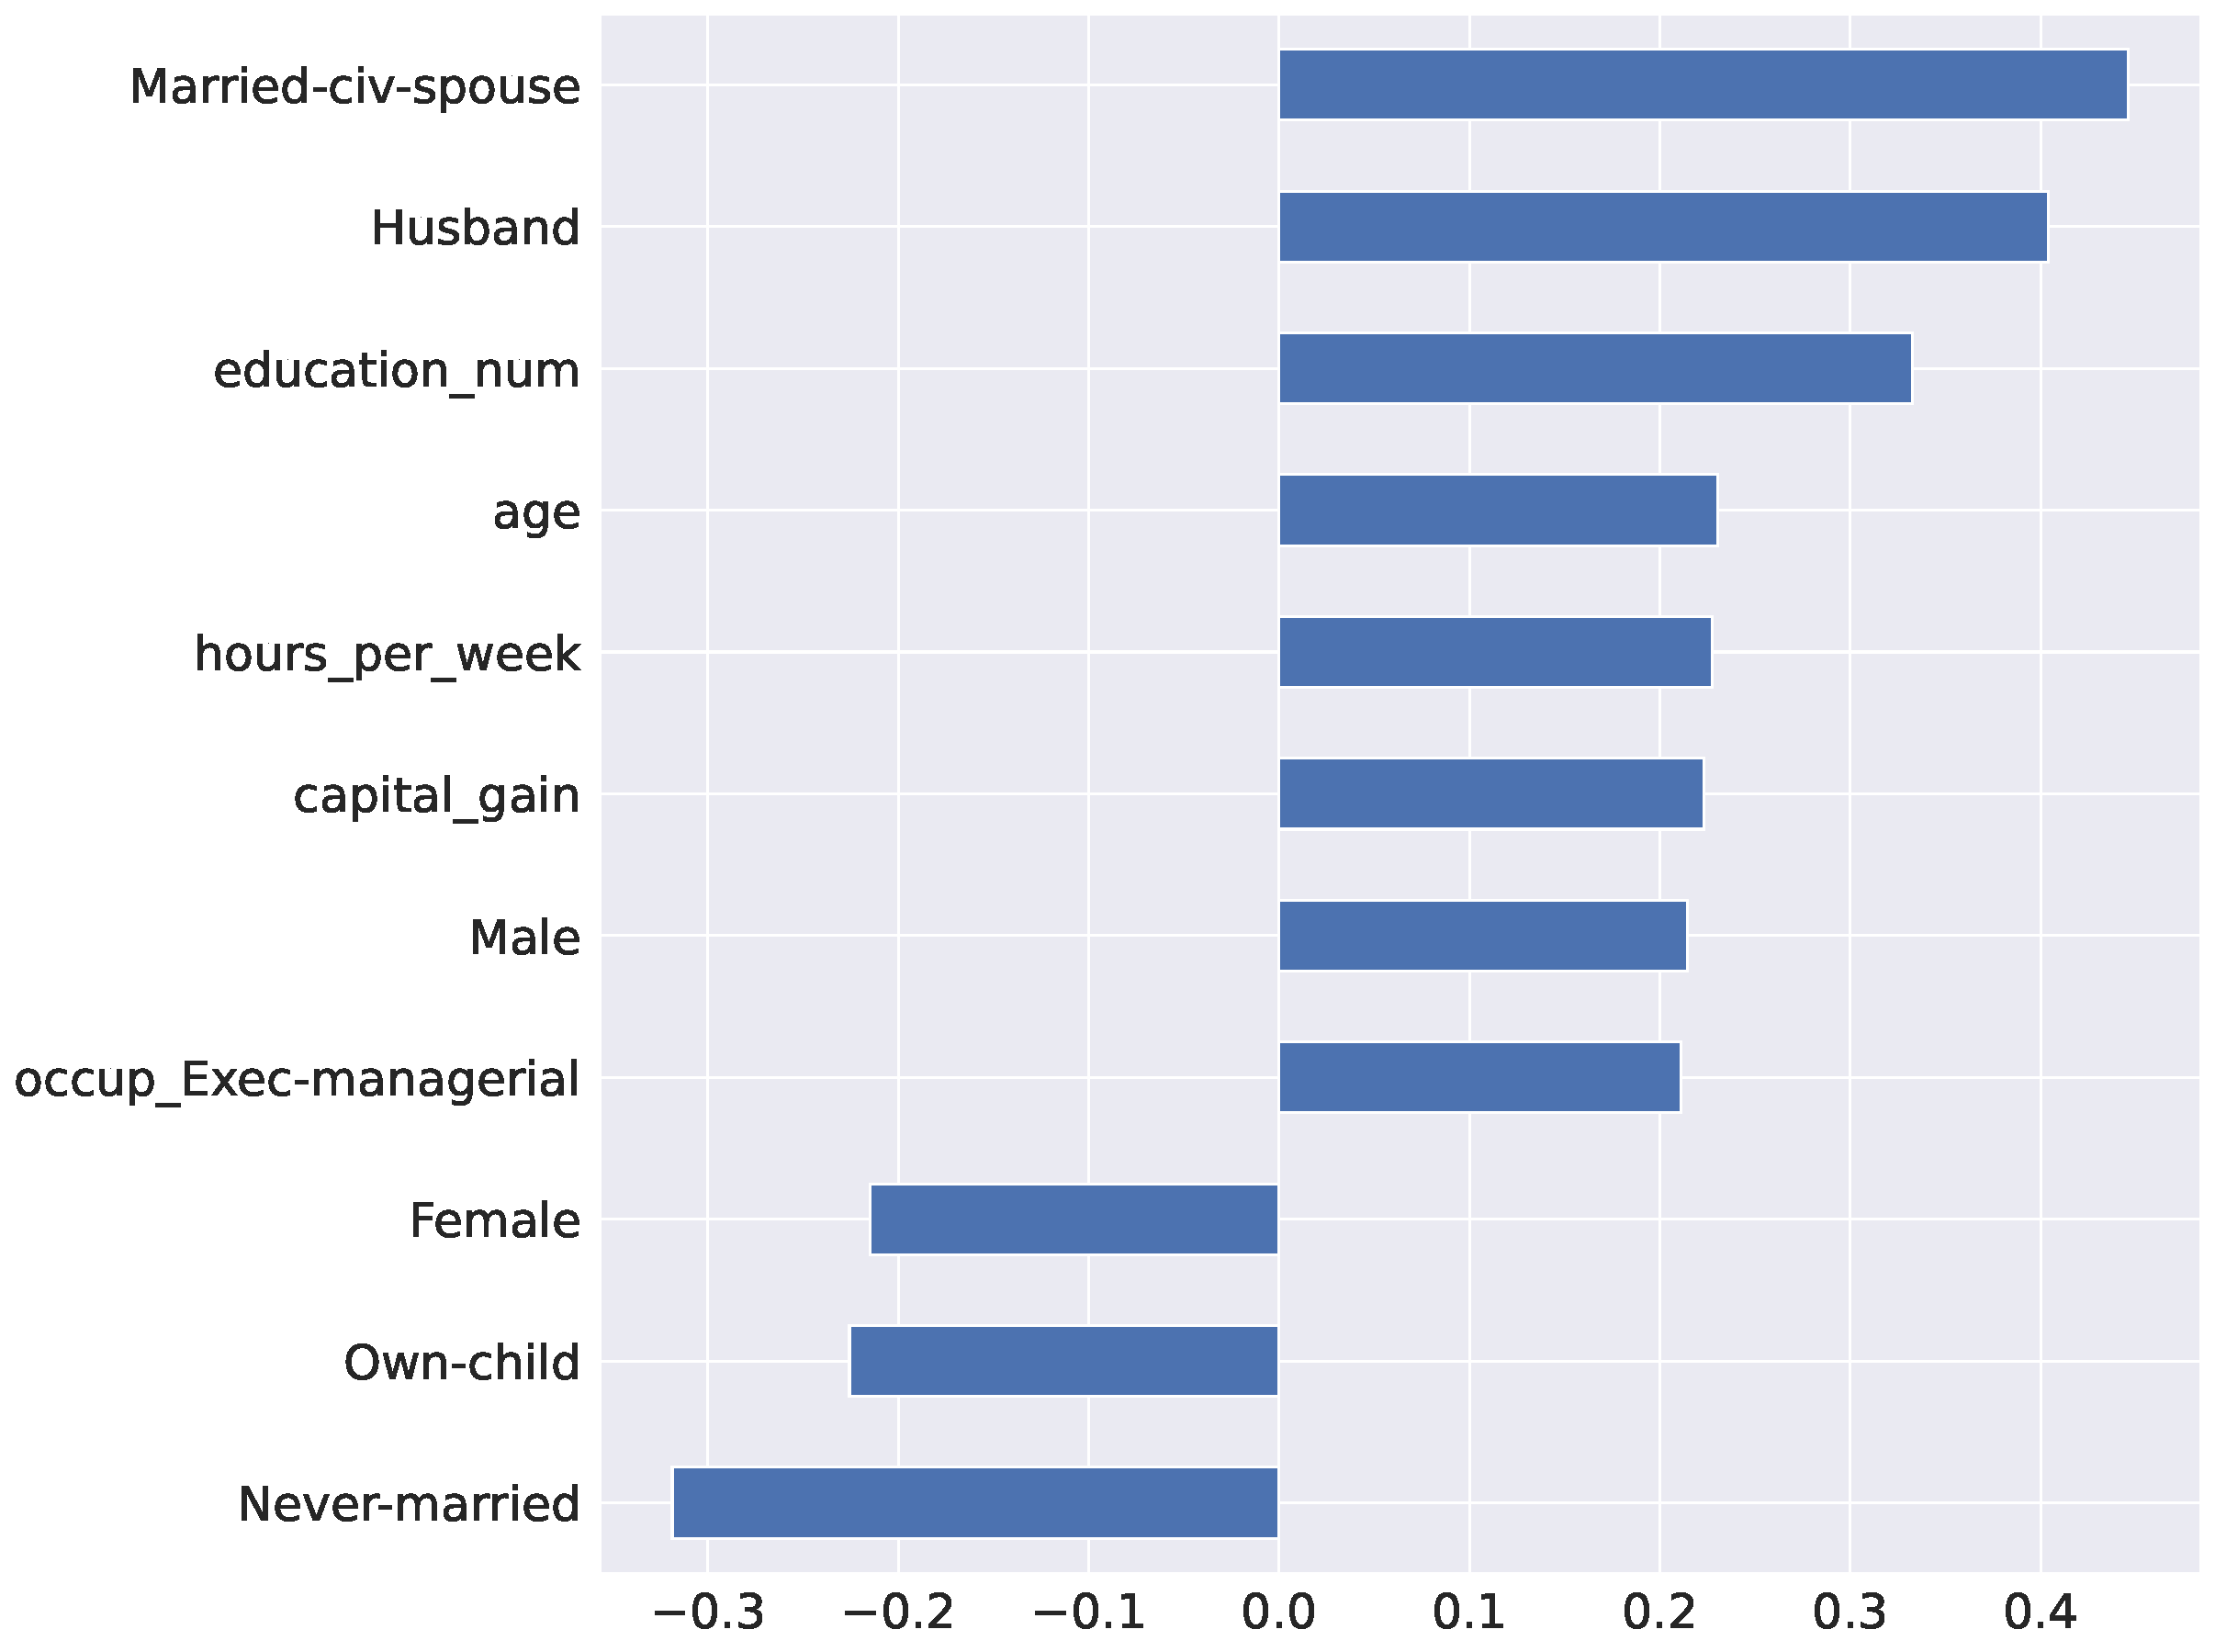
\includegraphics[width=.7\textwidth]{corr_with_target.pdf}
    \end{center}
    \caption{Variáveis que possuem correlação com a variável target com módulo superior a 0.2.}
    \label{fig: corr target}
\end{figure}
É possível observar, surpreendentemente, que as variáveis com maior correlação, tanto positiva quanto negativa, são relacionadas ao estado conjugal dos indivíduos.
Vemos que estar em um casamento com um civil está correlacionado positivamente com ganhar mais de \$50 000 por ano, enquanto nunca ter se casado está correlacionado negativamente.

É perceptível, também, que a característica \verb|Male| possui correlação positiva com target, enquanto \verb|Female| apresenta correlação negativa, indicando que, no geral, homens possuem salários melhores que mulheres.
Também podemos ver que trabalhar mais durante a semana, ser mais velho e ter uma educação melhor estão correlacionados positivamente com possuir um salário acima de \$50 000.

Com intuito de explorar mais essas relações, produzimos a Figura \ref{fig: hours age ed}.
Vemos que, à medida que o grau máximo de educação obtido aumenta, também aumenta a proporção de indivíduos que ganha mais de \$50 000 por ano.
Também percebemos que, no geral, poucas pessoas trabalham mais que 60 horas por semana, principalmente os mais velhos.

Por fim, também verificamos a distribuição da idade dos indivíduos, visualizando-a em conjunto com a variável \verb|target| na Figura \ref{fig: age}.
Podemos ver que as maiores proporções de indivíduos que ganham mais de \$50 000 são observadas entre 35 e 50 anos, aproximadamente.

\section{Próximos passos}

Na segunda parte desse trabalho, vamos ajustar modelos de classificação ao conjunto de dados escolhido, com o objetivo de prever o valor de \verb|target| para um dado indivíduo.
Para tanto, teremos que lidar de alguma forma com os dados faltantes, seja excluindo-os, ou aplicando técnicas estatísticas para preenchê-los artificialmente respeitando as características dos dados.
Esperamos conseguir interpretar os resultados obtidos, de modo a identificar quais variáveis são mais relevantes para determinar a renda de um indivíduo.

\begin{figure}[H]
    \begin{center}
        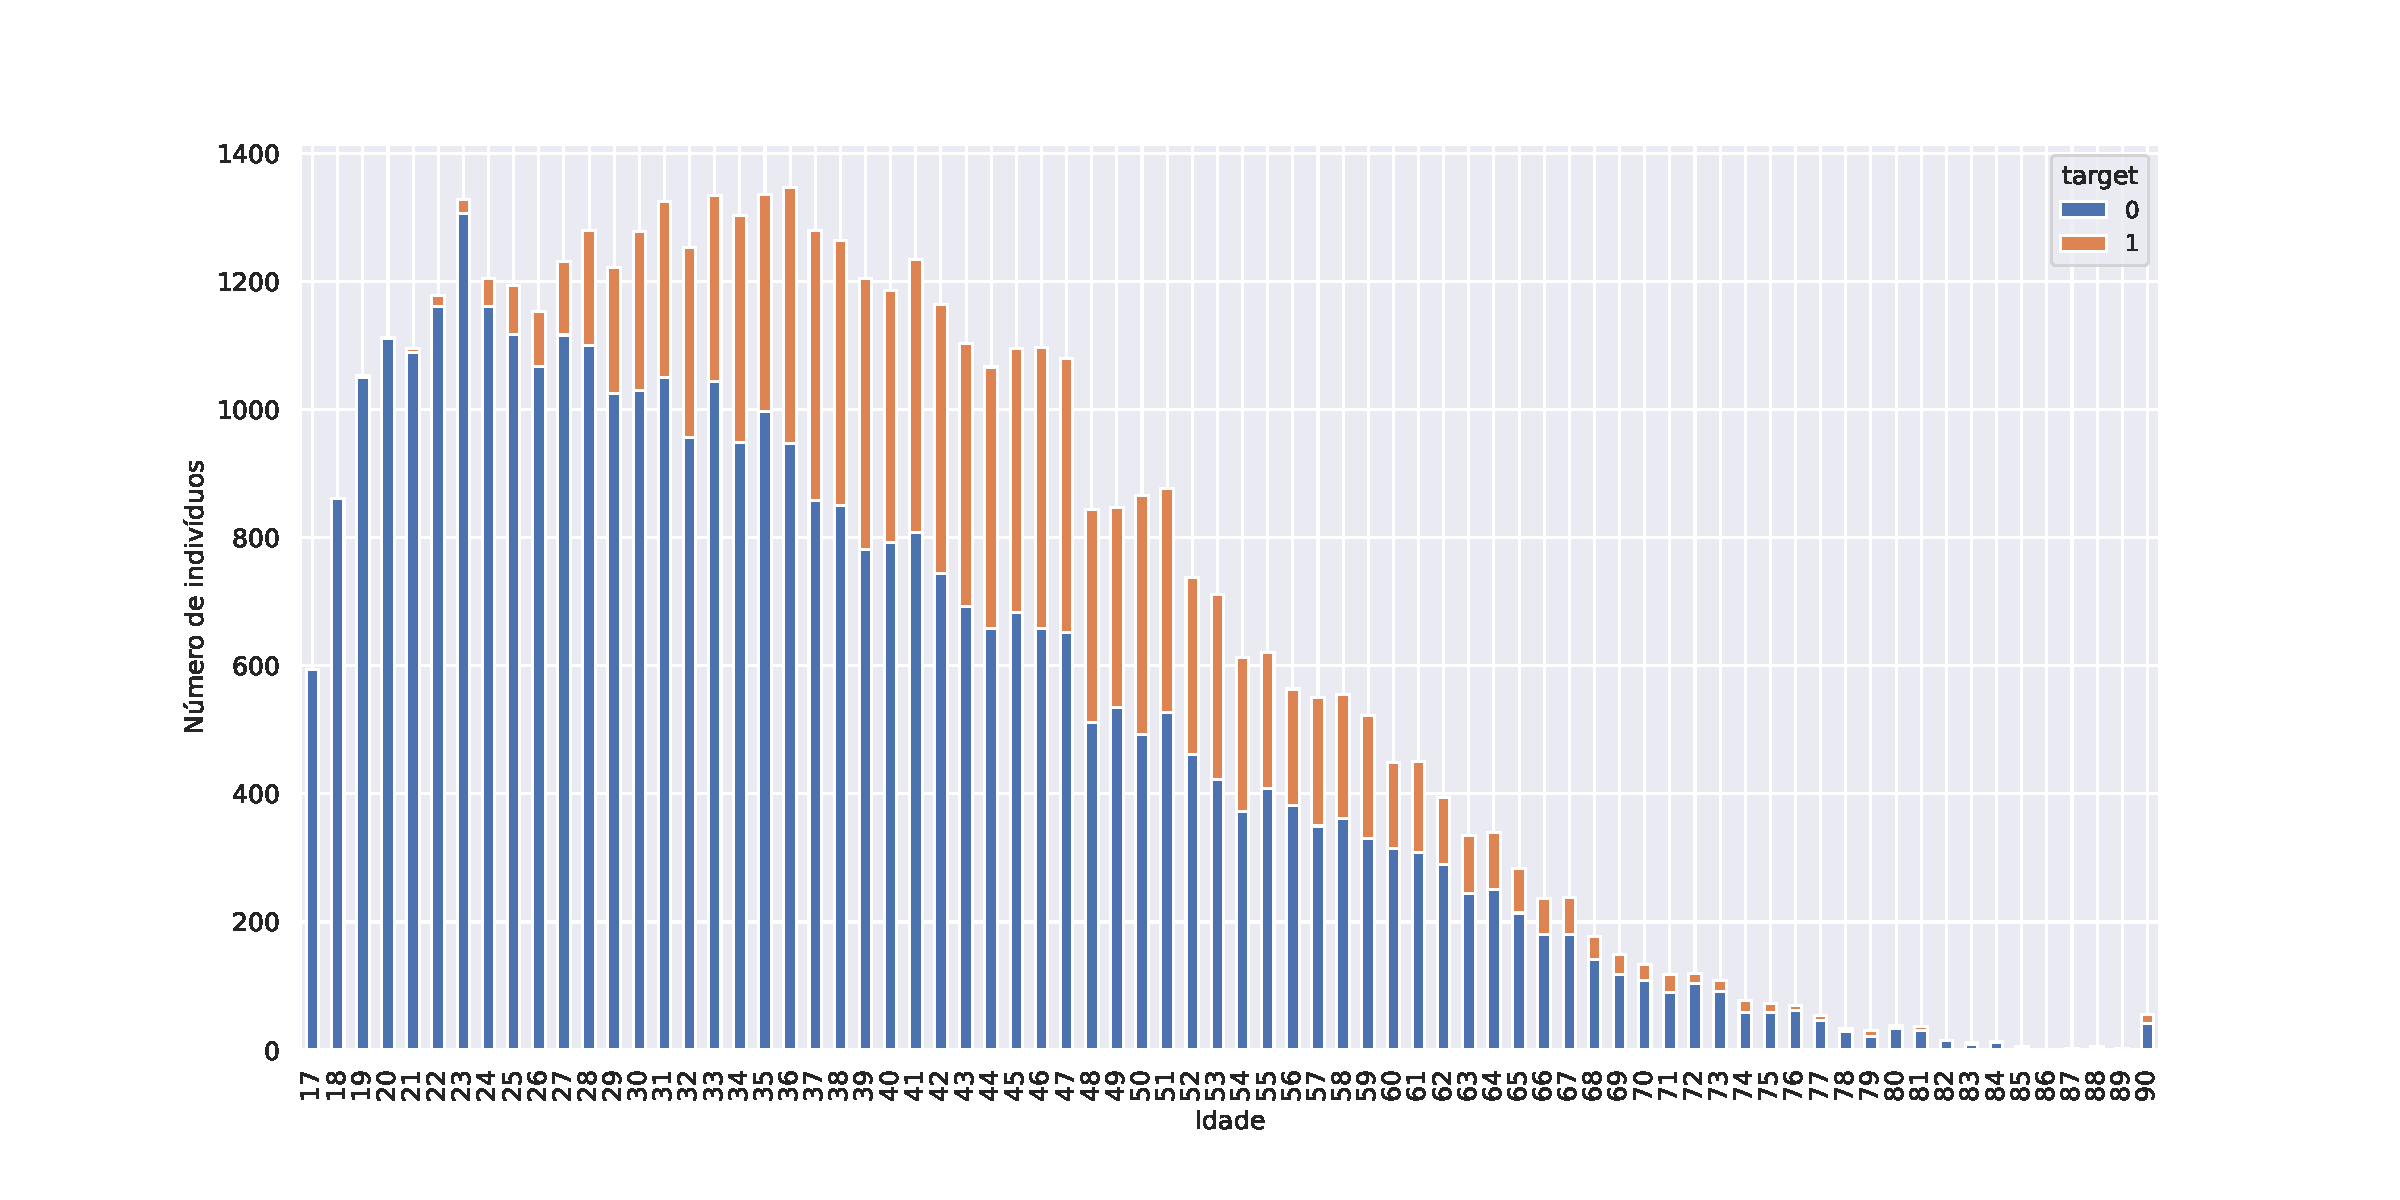
\includegraphics[width=\textwidth]{age.pdf}
    \end{center}
    \caption{Distribuição da idade dos indivíduos, discriminada por target.}
    \label{fig: age}
\end{figure}
\newpage
\begin{figure}[H]
    \begin{center}
        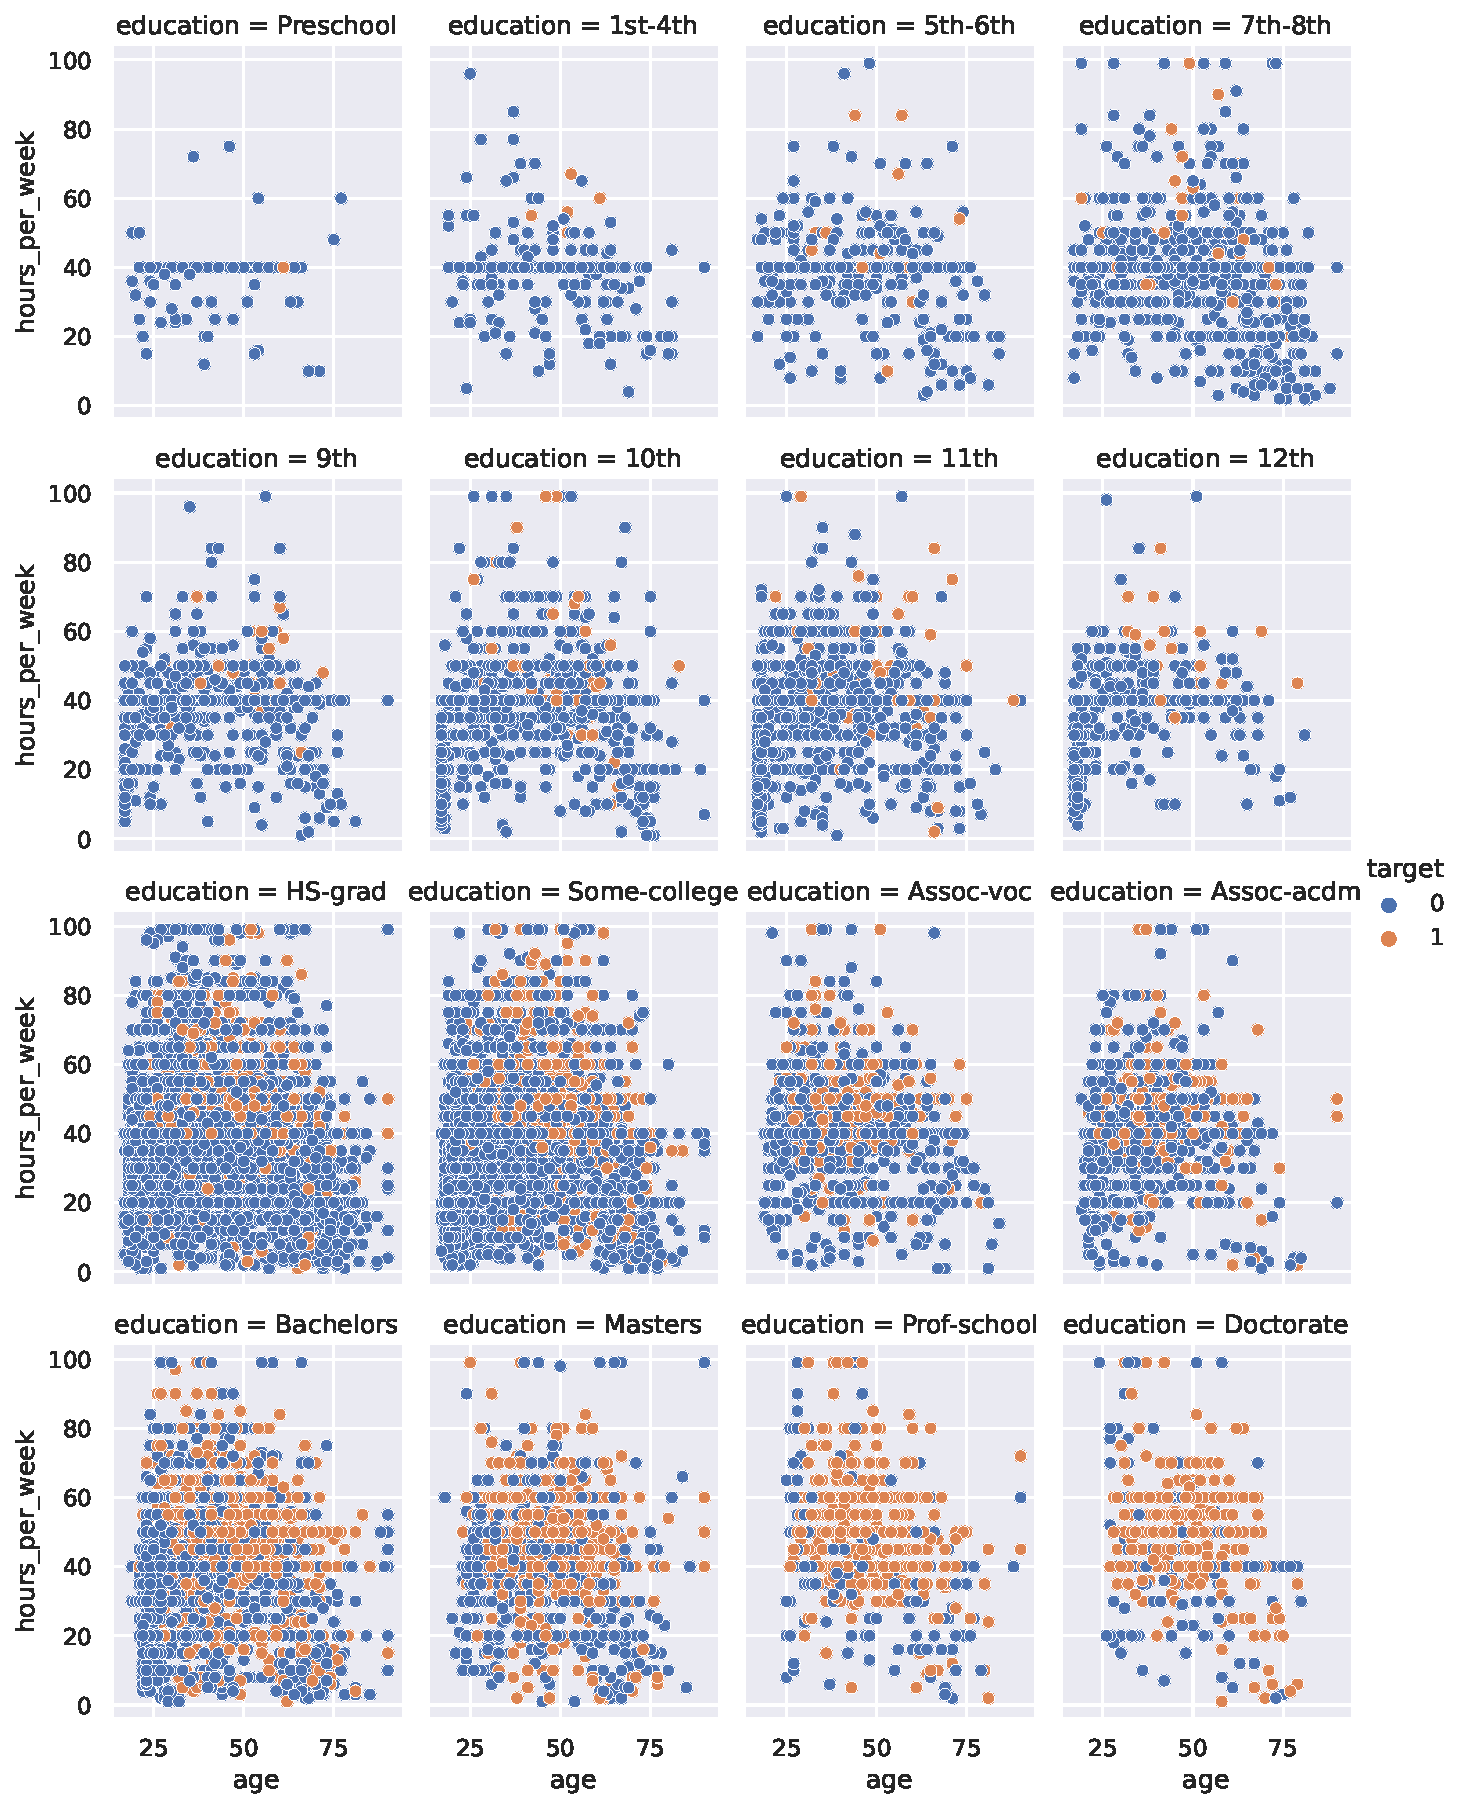
\includegraphics[width=\textwidth]{hours_age_by_ed.pdf}
    \end{center}
    \caption{Horas trabalhadas por semana e idade, observadas em diferentes níveis de formação educacional.}
    \label{fig: hours age ed}
\end{figure}

\printbibliography

\end{document}

